% GGUF k-quant super-block structure -- why it cannot serve as a controlled
% "4-bit" condition.
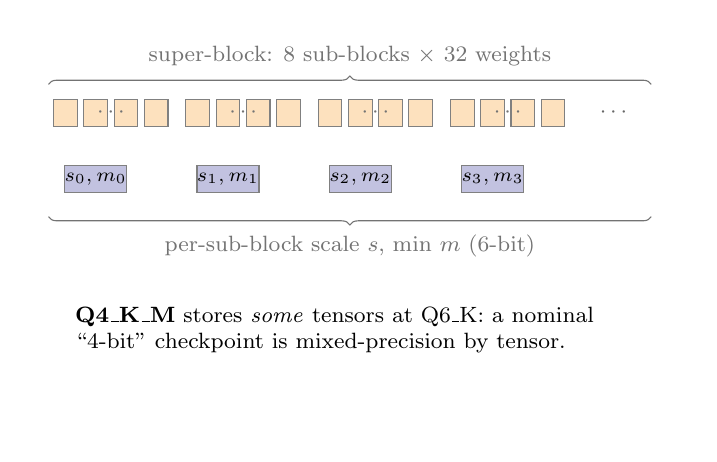
\begin{tikzpicture}[
  font=\fontsize{8}{9.6}\selectfont, x=1.2mm, y=1.2mm,
  wt/.style={draw=black!50, fill=BurntOrange!22, minimum width=3.0mm,
             minimum height=3.4mm, inner sep=0pt},
  sc/.style={draw=black!50, fill=NavyBlue!24, minimum width=6.2mm,
             minimum height=3.4mm, inner sep=0pt, font=\fontsize{7}{8}\selectfont},
  brace/.style={decorate, decoration={brace, amplitude=3pt}, black!55},
]
\useasboundingbox (-4,-34) rectangle (66,9);
% one super-block = 8 sub-blocks x 32 weights
\foreach \b in {0,...,3} {
  \foreach \i in {0,...,3} {
    \node[wt] at (\b*14 + \i*3.2, 0) {};
  }
  \node[font=\fontsize{8}{9.6}\selectfont, text=black!55] at (\b*14 + 4.8, 0) {$\cdots$};
  \node[sc] at (\b*14 + 3.2, -7) {\scriptsize $s_\b,m_\b$};
}
\node[font=\fontsize{8}{9.6}\selectfont, text=black!60] at (58, 0) {$\cdots$};
\draw[brace] (-1.8, 3.0) -- (62, 3.0)
  node[midway, above=3pt, font=\fontsize{8}{9.6}\selectfont]
  {super-block: 8 sub-blocks $\times$ 32 weights};
\draw[brace] (62, -11.0) -- (-1.8, -11.0)
  node[midway, below=3pt, font=\fontsize{8}{9.6}\selectfont]
  {per-sub-block scale $s$, min $m$ (6-bit)};
\node[font=\fontsize{8}{9.6}\selectfont, anchor=west, text width=68mm, align=left] at (0, -23)
  {\textbf{Q4\_K\_M} stores \emph{some} tensors at Q6\_K: a nominal
   ``4-bit'' checkpoint is mixed-precision by tensor.};

\end{tikzpicture}
